\chapter{实物平台实验验证}
\section{引言}
第5章在Gazebo仿真环境中建立了神经距离编码MPC与对比方法的统一实验协议。仿真环境的传感器噪声模型、障碍几何和底盘动力学均为理想化设定，无法反映真实激光雷达的量测稀疏与遮挡、定位漂移、通信延迟以及底盘执行偏差对局部规划的影响。因此，本章在自研移动机器人平台上开展实物实验，用于检验前述感知、定位与规划模块构成的导航软件链路在真实条件下能否稳定协同运行，并记录典型非凸障碍环境中的运行形态。

本章的证据定位与第5章不同：仿真实验承担不同方法在统一条件下的定量比较，实物实验承担真实平台上的部署可行性与运行稳定性验证，不复现仿真场景的完整统计对比。

\section{实验平台与运行环境}
实验采用自研移动机器人平台，搭载第2章所述Livox MID-360三维激光雷达，机载计算平台运行Ubuntu 20.04与ROS Noetic，实时定位由第3章基于FAST-LIO2与预建点云地图的定位模块提供，障碍检测与局部地图由第4章模块生成，局部规划控制频率为10\,Hz。该平台采用麦克纳姆轮全向底盘，与第5章仿真被控对象的运动学形式一致，实验中按式~\eqref{eq:ROS速度指令}的接口接收规划器输出的机体系两个平移速度分量与角速度，因此被控对象的实际运动与式~\eqref{eq:全向底盘离散运动模型}的建模假设保持一致。规划器所加载的距离编码器权重与仿真实验相同：编码器的输入输出仅由底盘轮廓尺寸决定，与仿真/实物的运行环境无关，因此无需为实物实验重新训练。

现有实物材料包含L型非凸障碍和多障碍组合两类环境。由于不同照片的障碍布局、机器人位置和拍摄范围并不完全一致，本章不将其排成“同一目标点下两种方法对比”或“连续导航过程”，而仅作为实验平台、典型障碍布局和运行状态的场景记录。

\begin{figure}[!htb]
	\centering
	\subfloat[L型非凸障碍场景]{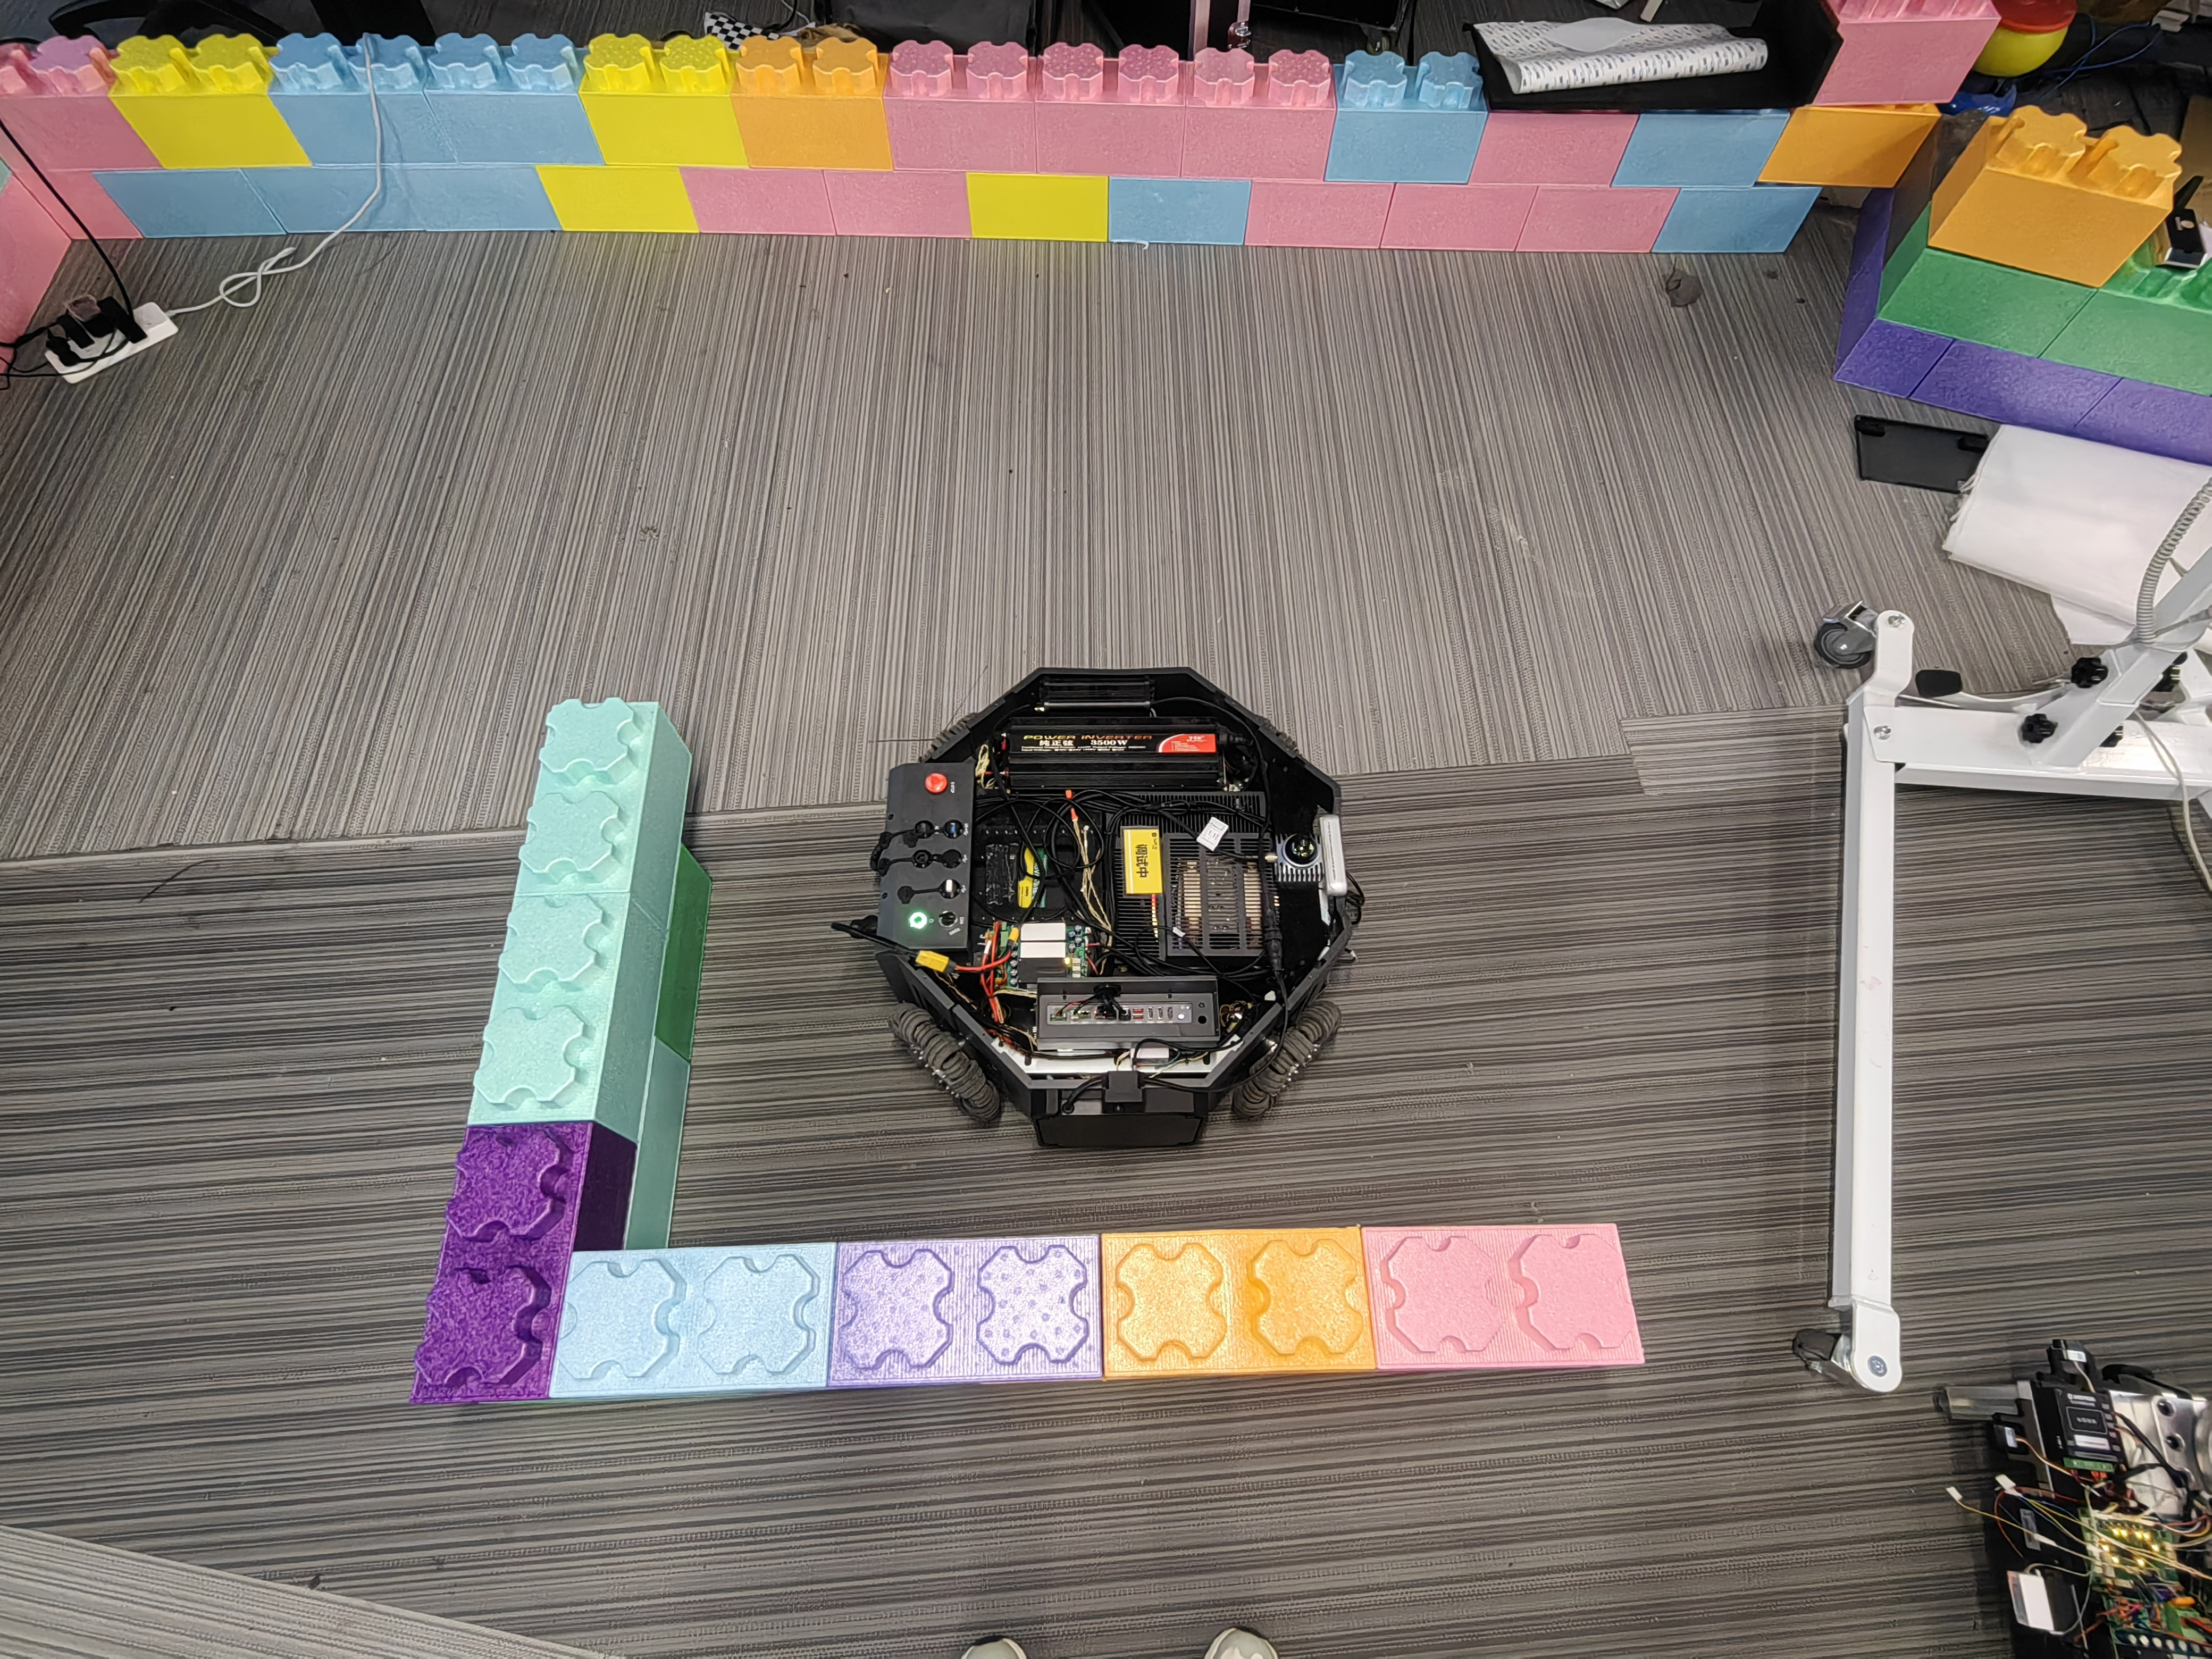
\includegraphics[width=0.48\textwidth]{pic/exp_goal1_neupan.jpg}}
	\hfill
	\subfloat[多障碍组合场景]{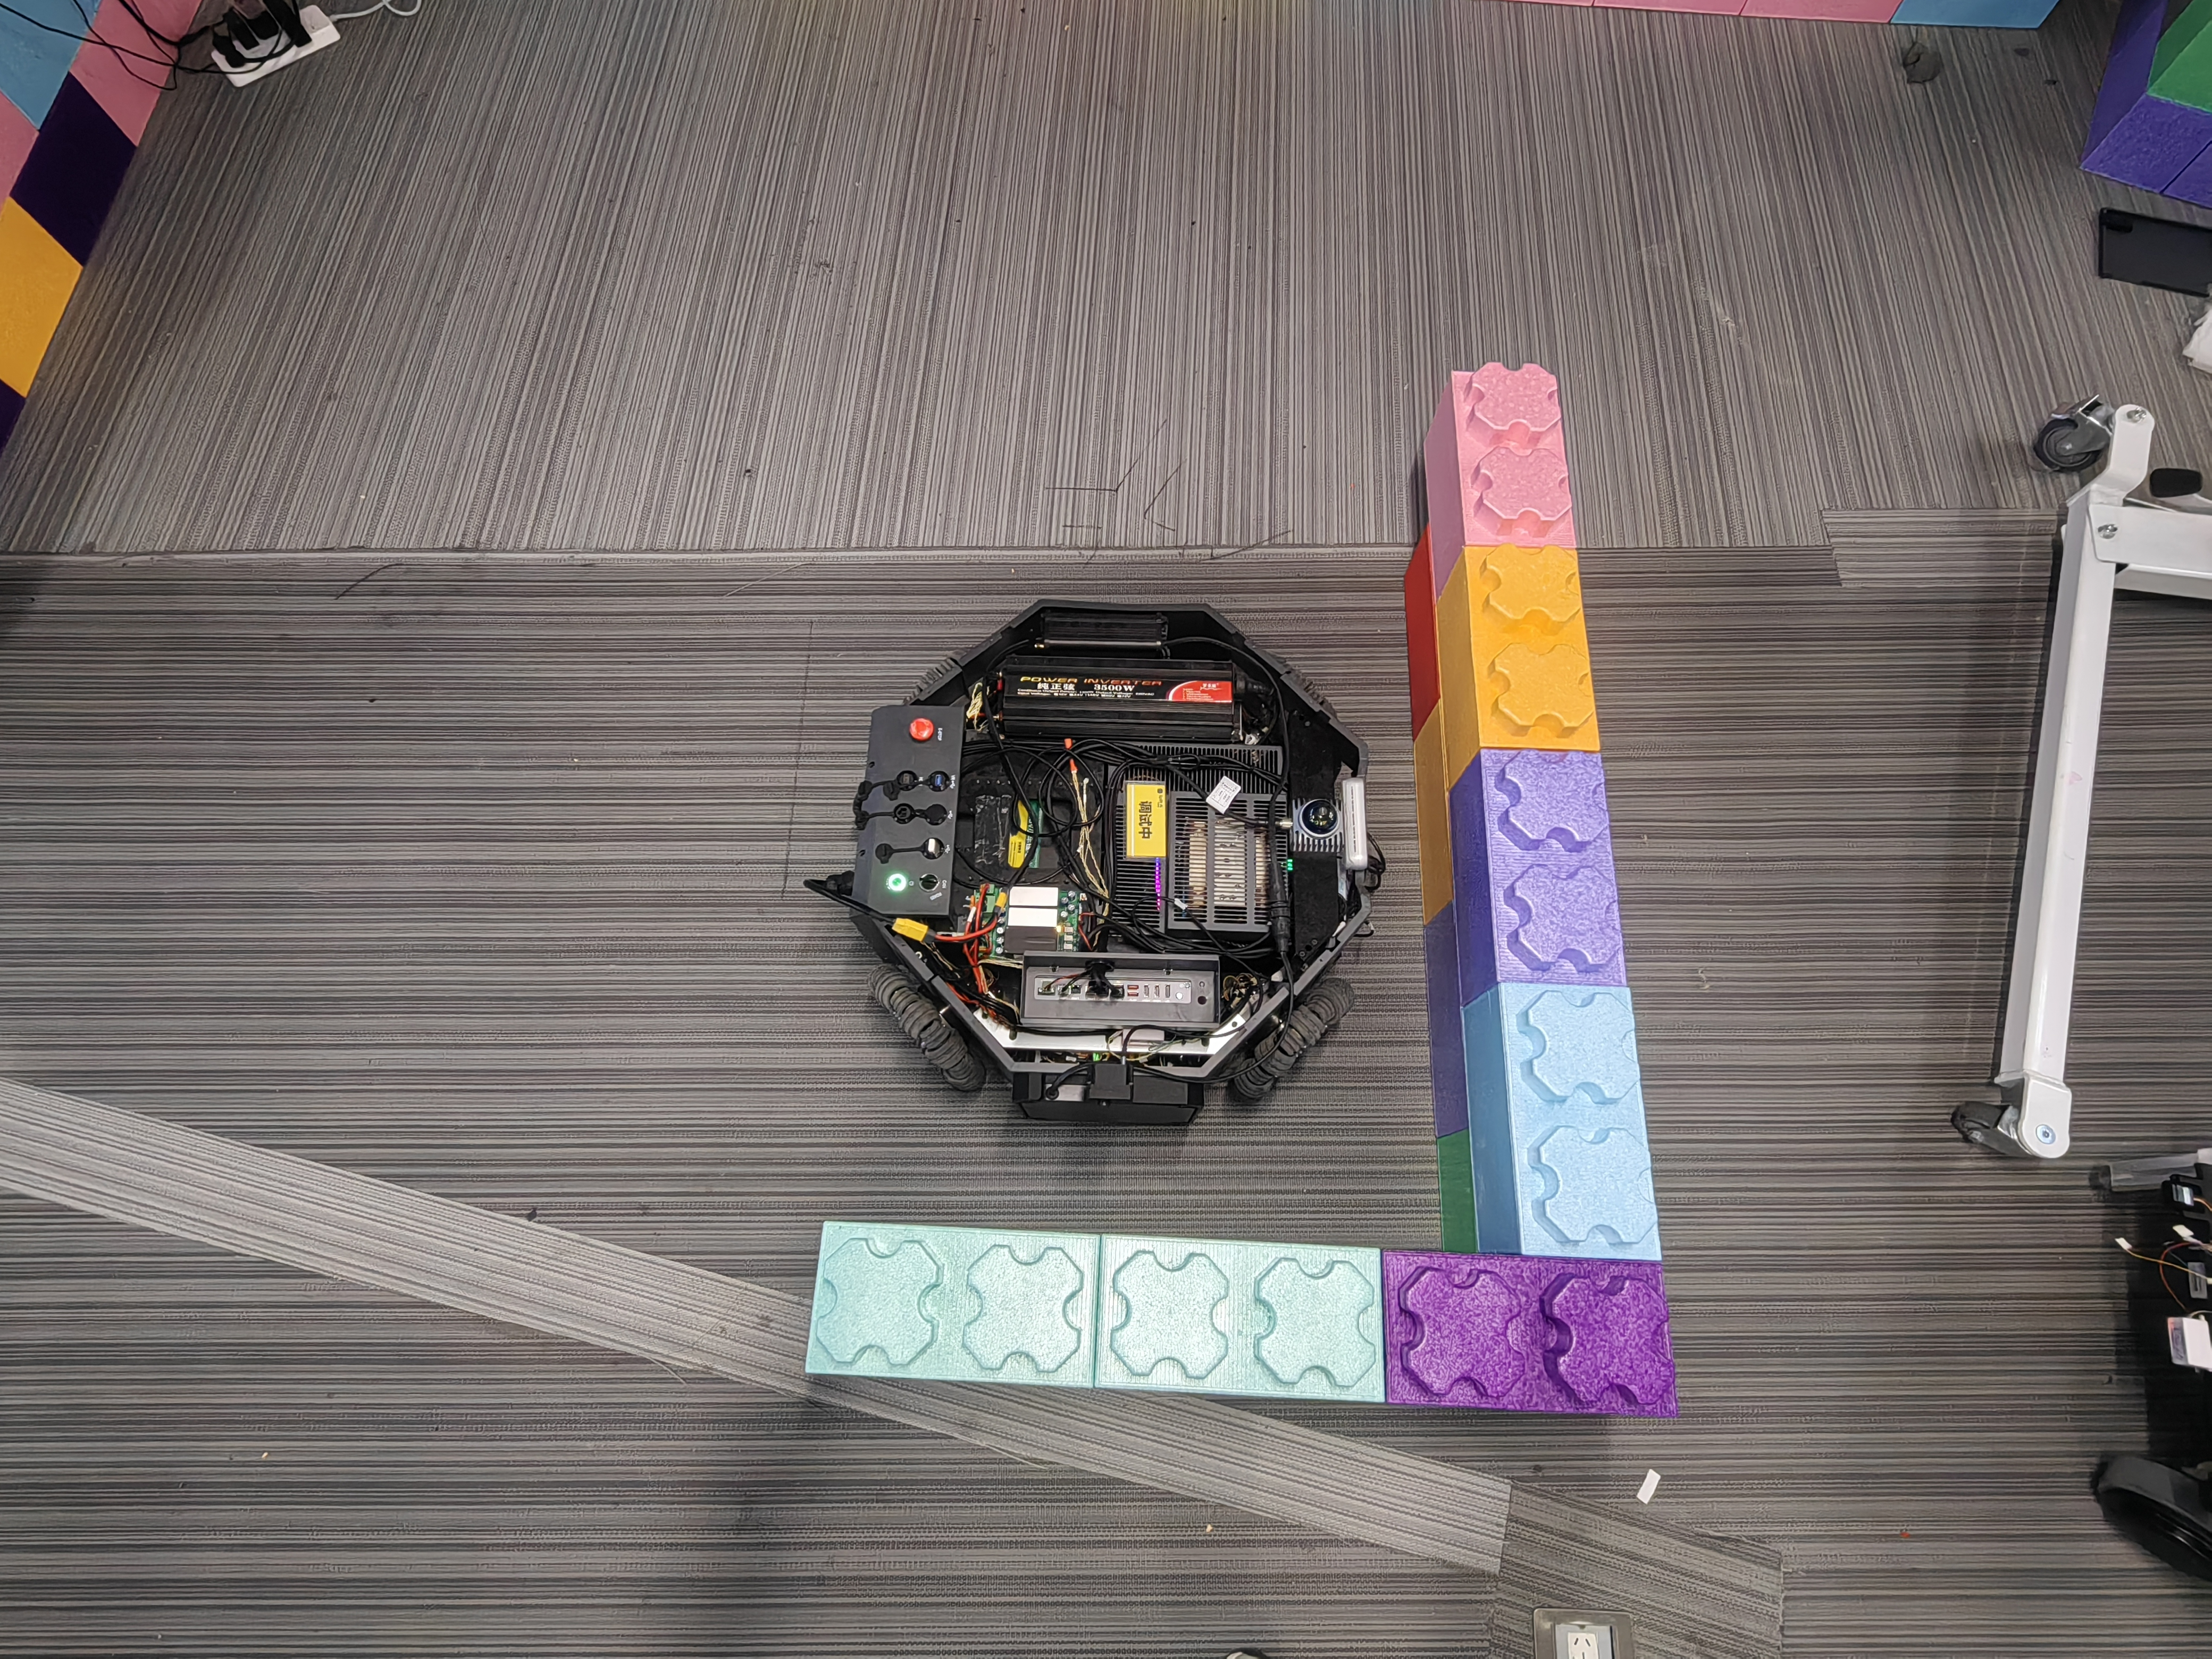
\includegraphics[width=0.48\textwidth]{pic/exp_goal2_neupan.jpg}}
	\caption{实物实验场景与机器人运行状态示例}
	\label{fig:实物实验场景示例}
\end{figure}

\section{L型非凸障碍运行验证}
L型场景将目标区域设置在障碍内凹侧，用于观察点级表示是否能够保留包络内部的真实可行空间。实物验证应以同一场次的ROS日志为准，在统一地图坐标系中叠加真实障碍轮廓、AABB包络、上层参考路径、机器人轨迹和起终点，并同步给出到目标距离、机体系速度及最小障碍距离曲线。现有照片只能证明平台和障碍场景已经搭建，不能替代同条件下的轨迹对照。

\begin{table}[!htb]
	\centering
	\caption{L型实物实验记录表（待同场次日志补充）}
	\label{tab:实物L型结果}
	\scriptsize
	\begin{tabular}{lccccc}
		\toprule
		方法 & 成功次数/总次数 & 终点误差/m & 任务时间/s & 最小距离/m & 平均规划耗时/ms \\
		\midrule
		AABB-MPC & 待填 & 待填 & 待填 & 待填 & 待填 \\
		本文方法 & 待填 & 待填 & 待填 & 待填 & 待填 \\
		\bottomrule
	\end{tabular}
\end{table}

在日志补齐前，本章只保留如下可核验的定性判断：AABB会将L型障碍的内凹部分包含在外接矩形内，因此可能压缩或阻断通向内部目标的可行空间；点级表示在感知边界质量足够时能够避免这一几何误判。是否成功到达、耗时多少以及两种方法差异是否显著，均应由同场次重复实验决定。

\section{复杂障碍环境运行展示与讨论}
多障碍组合照片用于展示规划器在更复杂真实环境中的运行形态。由于当前照片并非同一场景的连续帧，也缺少与AABB-MPC和DWA一一对应的同步日志，本节不据此计算成功率或宣称方法排序。后续若补采数据，应固定场景、起终点和传感器配置，分别运行三种方法，并按与仿真一致的指标生成轨迹与时序图。

真实环境相对仿真环境的主要差异有三点，也是后续补采数据时需重点记录的对象：一是激光雷达点云在障碍侧面与低矮结构上存在缺失，点级约束的有效性直接取决于边界点的完整程度；二是定位输出存在厘米级漂移与短时跳变，会同时影响参考路径截取与距离约束的几何基准；三是底盘存在加速度限制与执行滞后，规划输出的速度指令并非即时生效，可能放大逐次线性化的预测误差。

\section{本章小结}
本章在自研移动机器人平台上对第5章的神经距离编码MPC进行了实物验证部署，明确了传感器配置、定位来源、控制频率和速度指令接口，并说明地图系平移速度经一次平面旋转变换为机体系指令后由麦轮底盘执行，与第5章的建模假设及编码器权重完全一致。针对L型非凸障碍和多障碍组合两类环境，本章给出了实验方案、记录表结构和可核验的定性判断。

当前实物材料仅能证明平台与场景已搭建、软件链路可运行，尚缺少同场次的同步日志，因此本章不给出定量性能结论；所有待填项均须在正式提交前由真实实验日志替换。
